\documentclass{article}
\usepackage{settings}
%to write english paragraph \selectlanguage{language}
%to write english inline \textenglish{...}

\title{HW10}
\author{דורון שפיגל}
\date{15.04.24}

\begin{document}
\maketitle



\begin{Question}
נתונה שרשרת אטומים המרוחקים זה מזה במרחק ממוצע $a$. התנועה של כל אטום מתוארת באמצעות מתנד הרמוני כך שאטום נתון מקושר לשני השכנים הקרובים הנמצאים במרחק $a$ ממנו באמצעות קפיץ עם קבוע $k_{1}$ ולשני שכנים הרחוקים יותר הנמצאים במרחק $2a$ באמצעות קפיץ $k_{2}$.\\
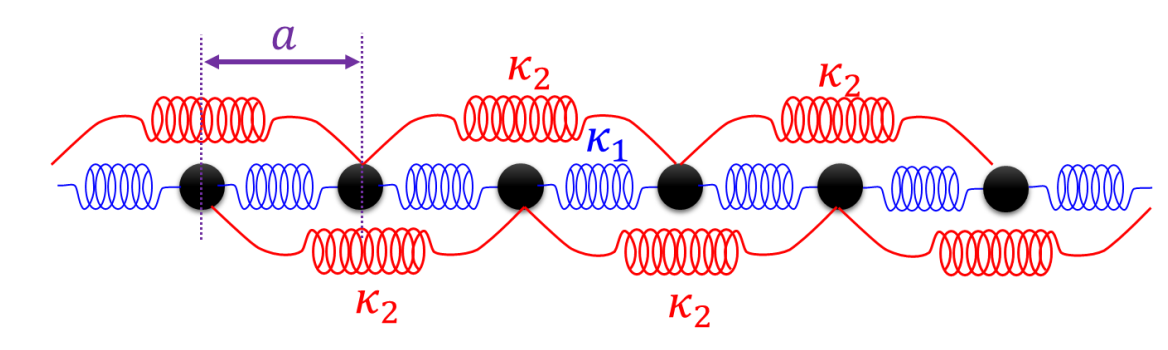
\includegraphics[width=0.9\textwidth]{Q1.png}\\
כמה אופנים אקוסטיים וכמה אופנים אופטיים ישנם במודל? מהו יחס הנפיצה במודל?\\
תחילה אגדיר תא יחידה, אני מחפש תא יחידה שיקיים מחזוריות בהזזה, לכן:\\
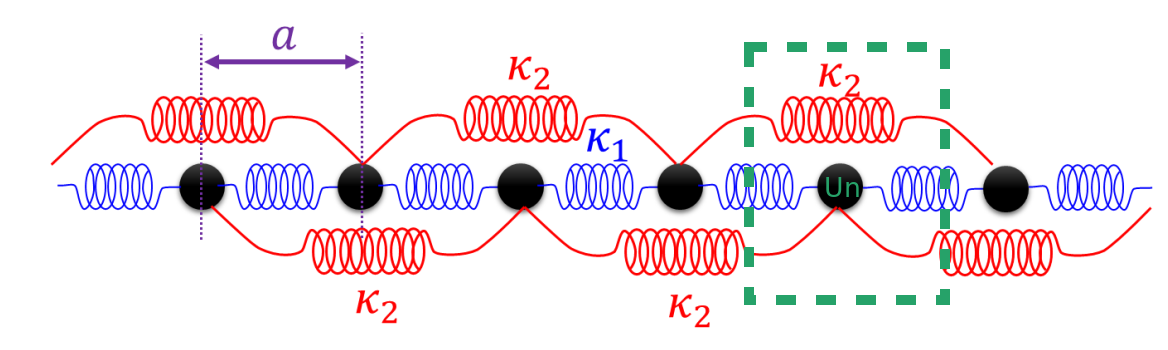
\includegraphics[width=0.9\textwidth]{Q1UnitCell.png}\\
יש לנו אטום יחיד בבעיה חד ממדית, לכן יש יחס נפיצה יחיד.\\
אקבל ביטוי לפוטנציאל:
\begin{align*}
    U_{1}&=0.5\cdot k_{1}\cdot\left( u_{n}-u_{n-1} \right)^{2}\\
    U_{2}&=0.5\cdot k_{1}\cdot\left( u_{n+1}-u_{n} \right)^{2}\\
    U_{3}&=0.5\cdot k_{2}\cdot\left( u_{n}-u_{n-2} \right)^{2}\\
    U_{4}&=0.5\cdot k_{2}\cdot\left( u_{n+2}-u_{n} \right)^{2}\\
\end{align*}
ולכן, הכוח:
\begin{align*}
    F&=-\od{U}{x}=\begin{cases}
        -k_{1}\left( u_{n}-u_{n-1} \right)\\
        k_{1}\left( u_{n+1}-u_{n} \right)\\
        -k_{2}\left( u_{n}-u_{n-2} \right)\\
        k_{2}\left( u_{n+2}-u_{n} \right)
    \end{cases}\\\rightarrow
    F&=
        k_{1} (- 2 u_{n} + u_{n+1} + u_{n-1})\\
        &+k_{2} (- 2 u_{n} + u_{n+2} + u_{n-2})
\end{align*}
נציב: $u_{n}=Ae^{i\left( kna-\omega(k) t \right)},\, F=m\od[2]{u}{t}=-m\ddot{u} $, ונקבל את יחס הנפיצה:
\begin{align*}
    -m\omega^{2}Ae^{i\left( kna-\omega(k) t \right)}&=
    k_{1}\cdot\left(
    -2Ae^{i\left( kna-\omega(k) t \right)}+Ae^{i\left( k(n+1)a-\omega(k) t \right)}
    +Ae^{i\left( k(n-1)a-\omega(k) t \right)}
    \right)\\
            &+
    k_{2}\cdot\left(
    -2Ae^{i\left( kna-\omega(k) t \right)}+Ae^{i\left( k(n+2)a-\omega(k) t \right)}
    +Ae^{i\left( k(n-2)a-\omega(k) t \right)}
    \right)\\
    \xrightarrow{\div Ae^{i\left( kna-\omega(k) t \right)}}-m\omega^{2}&=
    k_{1}\cdot\left( 
        -2+e^{ika}+e^{-ika}
    \right)+
    k_{2}\cdot\left( 
        -2+e^{2ika}+e^{-2ika}
    \right)\\
    \xrightarrow{\cos(A)=\frac{e^{iA}+e^{-iA}}{2}}-m\omega^{2}&=
    k_{1}\cdot\left( 
        -2+2\cos(ka)
    \right)+
    k_{2}\cdot\left( 
        -2+2\cos(2ka)
    \right)\\
    \xrightarrow{\times (-1)}m\omega^{2}&=
    k_{1}\cdot\left( 
        2-2\cos(ka)
    \right)+
    k_{2}\cdot\left( 
        2-2\cos(2ka)
    \right)\\&=
    2k_{1}\cdot\left( 
        1-\cos(ka)
    \right)+
    2k_{2}\cdot\left( 
        1-\cos(2ka)
    \right)\\
    \xrightarrow{2\sin^{2}(A)=1-\cos(2A)}m\omega^{2}&=
    2k_{1}\cdot\left( 
        2\sin^{2}\left( \frac{ka}{2} \right)
    \right)+
        2k_{2}\cdot\left( 
        2\sin^{2}\left( ka \right)
    \right)\\&=
        4k_{1}\cdot 
        \sin^{2}\left( \frac{ka}{2} \right)
    +
        4k_{2}\cdot 
        \sin^{2}\left( ka \right)\\
    \xrightarrow{\div m} \omega^{2}&=
    \frac{4}{m}k_{1}\cdot 
        \sin^{2}\left( \frac{ka}{2} \right)
    +
        \frac{4}{m}k_{2}\cdot 
        \sin^{2}\left( ka \right)\\
    \Rightarrow &\boxed{\omega(k)=\sqrt{
        \frac{4}{m}k_{1}\cdot 
        \sin^{2}\left( \frac{ka}{2} \right)
    +
        \frac{4}{m}k_{2}\cdot 
        \sin^{2}\left( ka \right)
    }}
\end{align*}
עבור $k\to0$, נקבל $\limit{k\to 0}{\omega(k)}=\sqrt{\frac{4}{m}k_{1}\cdot 0+\frac{4}{m}k_{2}\cdot 0}=0$, ולכן יש ענף אקוסטי. עם 2 אופנים.
%W=\sqrt{\frac{4}{m}k_{1}\cdot \sin^{2}\left( \frac{ka}{2} \right)+\frac{4}{m}k_{2}\cdot \sin^{2}\left( ka \right)}
%simplify(var["W"]) = 2*sqrt((k_1*sin(a*k/2)**2 + k_2*sin(a*k)**2)/m)
%AtomicExpr(separatevars(approx_sin(var["W"], LATEX=False),[k],  force=True, dict=True)['coeff']) = AtomicExpr(a*sqrt(k_1 + 4*k_2)/sqrt(m))
%collect(approx_sin(var["W"], LATEX=False), k**2) = sqrt(k**2*(a**2*k_1/m + 4*a**2*k_2/m)) = sqrt(k**2*(a**2*k_1/m + 4*a**2*k_2/m))
%Symbol('k', positive=True, integer=True) = k
%var["W"] = sqrt(4*k_1*sin((a*k)/2)**2/m + 4*k_2*sin(a*k)**2/m)
%print(type(var["W"])) = None
%print(var["W"])  = None
%Vsound(var["W"]) = 
%diss(var["W"], k)
\begin{align*}
    %Vsound(var["W"]) = 
    \omega(k)&\approx\sqrt{\frac{a^{2} k^{2} k_{1}}{m} + \frac{4 a^{2} k^{2} k_{2}}{m}}=\frac{a \sqrt{k_{1} + 4 k_{2}}}{\sqrt{m}}\times k\\\rightarrow  V_{sound}&=\frac{a \sqrt{k_{1} + 4 k_{2}}}{\sqrt{m}}\\
    %latex(trigsimp(diff(var["W"], k))) = 
    &=\frac{a (k_{1} + 4 k_{2} \cos{(a k)}) \sin{(a k)}}{2 m \sqrt{\frac{k_{1} \sin^{2}{(\frac{a k}{2})} + k_{2} \sin^{2}{(a k)}}{m}}} = \frac{a (k_{1} + 4 k_{2} \cos{(a k)}) \sin{(a k)}}{2 m \sqrt{\frac{k_{1} \sin^{2}{(\frac{a k}{2})} + k_{2} \sin^{2}{(a k)}}{m}}} \\ = 
    V_{g}&=\frac{\frac{2 a k_{1} \sin{(\frac{a k}{2})} \cos{(\frac{a k}{2})}}{m} + \frac{4 a k_{2} \sin{(a k)} \cos{(a k)}}{m}}{\sqrt{\frac{4 k_{1} \sin^{2}{(\frac{a k}{2})}}{m} + \frac{4 k_{2} \sin^{2}{(a k)}}{m}}}\\
    a=\frac{2 a k_{1} \sin{(\frac{a k}{2})} \cos{(\frac{a k}{2})}}{m}\\
    b=\frac{4 a k_{2} \sin{(a k)} \cos{(a k)}}{m}\\
    latex(trigsimp(var["a"])) = \frac{a k_{1} \sin{(a k)}}{m}\\
    latex(trigsimp(var["b"])) = \frac{2 a k_{2} \sin{(2 a k)}}{m}
\end{align*}




\end{Question}











\end{document}